\documentclass[zihao=false,fontset=windows]{ctexart}
% ctexart 不接受任意 pt 选项。正文改 {10pt}，方括号里是行距。
\usepackage{scrextend}
\changefontsizes[12pt]{10pt}

\usepackage[a4paper,left=2.35cm,right=2.35cm,top=1.7cm,bottom=1.9cm]{geometry}
\usepackage{xcolor}
\usepackage{graphicx}
\usepackage{amsmath,amssymb}
\usepackage{enumitem}
\usepackage{tabularx}
\usepackage{colortbl}
\usepackage{listings}
\usepackage{hyperref}
\usepackage[most]{tcolorbox}

\definecolor{feishuText}{RGB}{31,35,41}
\definecolor{feishuBlue}{RGB}{36,91,219}
\definecolor{feishuRed}{RGB}{216,57,49}
\definecolor{feishuGray}{RGB}{100,106,115}
\definecolor{feishuGray2}{RGB}{143,149,158}
\definecolor{feishuPinkBg}{RGB}{251,191,188}
\definecolor{quoteBar}{RGB}{51,112,255}
\definecolor{codebg}{RGB}{245,246,247}
\definecolor{codeborder}{RGB}{222,224,227}
\definecolor{inlinebg}{RGB}{242,243,245}
\definecolor{callRed}{RGB}{253,226,226}
\definecolor{callOrange}{RGB}{255,245,235}
\definecolor{callYellow}{RGB}{254,255,240}
\definecolor{callGreen}{RGB}{240,251,239}
\definecolor{callBlue}{RGB}{240,244,255}
\definecolor{callRedSoft}{RGB}{254,241,241}
\definecolor{callSun}{RGB}{255,255,204}
\definecolor{tableHead}{RGB}{242,243,245}
\definecolor{tableRule}{RGB}{222,224,227}
\definecolor{codeText}{RGB}{31,35,41}
\definecolor{codeKeyword}{RGB}{0,0,255}
\definecolor{codeComment}{RGB}{0,128,0}
\definecolor{codeString}{RGB}{163,21,21}

\setmainfont{Times New Roman}
\setCJKmainfont{Microsoft YaHei}[AutoFakeBold=2.2]
\setCJKsansfont{Microsoft YaHei}[AutoFakeBold=2.2]
\setCJKmonofont{Microsoft YaHei}[AutoFakeBold=2.2]
\setmonofont{Consolas}
\newfontfamily\emojifont{Segoe UI Emoji}

\hypersetup{
  colorlinks=true,
  urlcolor=feishuBlue,
  linkcolor=feishuBlue,
  unicode=true,
  pdftitle={DeepSeek-V4.1-Flash 架构：技术报告/源码解析}
}

\setlength{\parindent}{0pt}
\setlength{\parskip}{0.42em}
\setlength{\fboxsep}{1.5pt}
\setlength{\emergencystretch}{3em}
\linespread{1.28}
\color{feishuText}
\arrayrulecolor{tableRule}
\urlstyle{same}

\setlist[enumerate]{label=\textcolor{feishuBlue}{\arabic*.}, leftmargin=1.7em, itemsep=0.22em, topsep=0.28em, parsep=0.08em, partopsep=0pt}
\setlist[itemize,1]{label=\textcolor{feishuBlue}{\textbullet}, leftmargin=1.35em, itemsep=0.18em, topsep=0.25em, parsep=0.06em, partopsep=0pt}
\setlist[itemize,2]{label=\textcolor{feishuBlue}{◦}, leftmargin=1.45em, itemsep=0.12em, topsep=0.15em}
\setlist[itemize,3]{label=\textcolor{feishuBlue}{\rule[0.18em]{0.38em}{0.38em}}, leftmargin=1.55em, itemsep=0.1em, topsep=0.12em}

\newcommand{\feiEmoji}[1]{{\emojifont #1}}
\newcommand{\incode}[1]{\colorbox{inlinebg}{\ttfamily\small #1}}
\newcommand{\bigmath}[1]{%
  \begin{center}\large$\displaystyle #1$\end{center}%
}

\lstset{
  language=Python,
  basicstyle=\ttfamily\footnotesize\color{codeText},
  keywordstyle=\color{codeKeyword},
  commentstyle=\color{codeComment},
  stringstyle=\color{codeString},
  showstringspaces=false,
  breaklines=true,
  columns=fullflexible,
  keepspaces=true,
  tabsize=4,
  upquote=true,
  aboveskip=2pt,
  belowskip=0pt,
  xleftmargin=0pt,
  frame=none
}

\tcbset{
  feishubase/.style 2 args={
    enhanced,
    boxrule=0pt,
    arc=8pt,
    left=10pt,
    right=10pt,
    top=7pt,
    bottom=7pt,
    before skip=6pt,
    after skip=6pt,
    colback=#1,
    colframe=#1,
    before upper={\feiEmoji{#2}\hspace{0.45em}\ignorespaces}
  }
}
\newtcolorbox{feishubox}[2]{feishubase={#1}{#2}, breakable}
\newtcolorbox{feishuboxnb}[2]{feishubase={#1}{#2}}

\newtcolorbox{feishuquote}{
  enhanced,
  breakable,
  boxrule=0pt,
  leftrule=3pt,
  arc=0pt,
  colframe=quoteBar,
  colback=white,
  left=8pt,
  right=2pt,
  top=2pt,
  bottom=2pt,
  before skip=4pt,
  after skip=4pt,
  before upper=\color{feishuGray}
}

\newtcolorbox{feishucode}{
  enhanced,
  breakable,
  colback=codebg,
  colframe=codeborder,
  boxrule=0.6pt,
  arc=6pt,
  left=6pt,
  right=6pt,
  top=5pt,
  bottom=4pt,
  before skip=6pt,
  after skip=6pt
}


\usepackage{needspace,longtable,array,adjustbox}
% 来源：https://scnajei2ds6y.feishu.cn/wiki/StxKwYlBfi7D0DkwO0rcdjMInEZ
% 按用户要求省略全部代码块；正文公式按网页渲染人工转写核对。
% 图24从页面已观察PNG资源导出；其他图以正常浏览器截图保留，详见复刻说明。
\begin{document}
{\zihao{1}\bfseries DeepSeek-V4.1-Flash 架构：\\技术报告/源码解析\par}

% source-block: 2 Q6zPdsIOgoXQTDxHYOUceflrneb quote_container
\begin{feishuquote}

% source-block: 3 JOyadS7Uco4j57xJWencQNnGnLh text
以下部分链接需要《大模型》笔记访问权限\par
\end{feishuquote}

% source-block: 4 doxcnemyK8Cir0q3e4CqHCv6J0f callout
\begin{feishubox}{callOrange}{📌}

% source-block: 5 doxcnYnzPYPXyL3fjBwgQkPVFie text
论文：\href{https://www.alphaxiv.org/pdf/2609.deepseek-v4-1-flash}{《DeepSeek-V4.1-Flash: Pushing the Limits of KV Cache Compression》}\par

% source-block: 6 doxcnJKEBlHBwa3OUmhRPXfux4e text
模型仓库：\href{https://huggingface.co/deepseek-ai/DeepSeek-V4.1-Flash}{deepseek-ai/DeepSeek-V4.1-Flash}\par

% source-block: 7 doxcn09CtjObjt87Qiv80YNnmUf text
推荐阅读：\par

% source-block: 8 doxcnbm7WPCDOfizkgyPc0o2Xmc text
\feiEmoji{🌟}\feiEmoji{🌟}\feiEmoji{🌟}\feiEmoji{🌟}\feiEmoji{🌟} \href{https://my.feishu.cn/wiki/UsuawakRYiqacxkD9vxcKzylnoe}{DeepSeek-V4 架构：技术报告/源码解析}\par

% source-block: 9 doxcnmd9YyYceDmK07yyaWy6JHc text
\feiEmoji{🌟}\feiEmoji{🌟}\feiEmoji{🌟}\feiEmoji{🌟}\feiEmoji{🌟} \href{https://scnajei2ds6y.feishu.cn/wiki/WsaawrdO3ifrmTk3ab4cSgjBnRb}{mHC：Manifold-Constrained Hyper-Connections}\par

% source-block: 10 doxcn0VmrWPx6Fhq6RR8L2Vn9he text
\feiEmoji{🌟}\feiEmoji{🌟}\feiEmoji{🌟}\feiEmoji{🌟} \href{https://scnajei2ds6y.feishu.cn/wiki/JwXTw0oUeimyoBk2QIgcSfBfn9g}{Engram：Conditional Memory via Scalable Lookup}\par

% source-block: 11 doxcn6K4NiKPGjqKnfgW7f4YLQc text
\feiEmoji{🌟}\feiEmoji{🌟}\feiEmoji{🌟} \href{https://scnajei2ds6y.feishu.cn/wiki/Hcj2wGTJEiohTikkdEKc7H4Nnlb}{Muon 优化器}\par

% source-block: 12 doxcn4fnwA6W3QvkwiqfUvqZxbN text
\feiEmoji{🌟}\feiEmoji{🌟} \href{https://scnajei2ds6y.feishu.cn/docx/MVsAdBXHVoE6FyxG16Kc6ee9noc}{DeepSeek V4多模态：Thinking with Visual Primitives}\par
\end{feishubox}

% source-block: 13 doxcnAVH9uCcJPZ0jxGxZDaJuUc callout
\begin{feishubox}{callOrange}{🤔}

% source-block: 14 doxcn4qFFaGr7cr1hlfCKyZsHfg text
DeepSeek-V4.1-Flash 相对 \href{https://my.feishu.cn/wiki/Gg57wvxiriwum6kVSlkctRy0nRh}{DeepSeek-V4} 的核心改进：\par
\begin{itemize}
\item 
% source-block: 15 doxcnTGv2JBZHqtcit4bPCiVGid bullet
\textcolor{feishuRed}{\textbf{CED（Causal Encoder-Decoder）}}：语言模型主干包括 20 层 Causal Encoder + 20 层 Decoder，Decoder 的全局 KV 由 Causal Encoder 最后一层 $H_{L/2}$ 投影得到，Prefill 的 FLOPs 大致减半。\par
\item 
% source-block: 16 doxcnNx7WeDFW9SM3ekBUZSpLWg bullet
\textcolor{feishuRed}{\textbf{CSA2（Compressed Sparse Attention 2）}}：简化了 \href{https://my.feishu.cn/wiki/Gg57wvxiriwum6kVSlkctRy0nRh}{DeepSeek-V4} CSA 的 KV 压缩建模，并且通过 Full / Reindex / Reuse 三种模式跨层共享 main KV / indexer K / Top-K Indices。\par
\item 
% source-block: 17 doxcn52Q4565zgT1WKWsIIsoDme bullet
\textcolor{feishuRed}{\textbf{Hierarchical Sparse Indexer}}：Decoder 的第一个 Full 层额外做 block-wise 候选池选择，Decoder 第二层开始的 Reindex 层只在候选池里打分，深层 Indexer 打分计算量不再随上下文增长。\par
\item 
% source-block: 18 doxcnQ3MVcztOqFgep8RgnNVkkg bullet
\textcolor{feishuRed}{\textbf{Engram}}：Engram 以每个位置结尾的 n-gram 为 Key 查询嵌入表，取回的记忆向量经门控写回残差流，本质上是静态知识的检索，不占用 Attention 与 FFN 的计算。\par
\item 
% source-block: 19 doxcnXcVgdpy8VEOGa1viis7kUf bullet
\textcolor{feishuRed}{\textbf{Single-Pass mHC、DSpark、head-wise Muon、FP4 main KV cache}}：mHC 消除 kernel 间依赖，投机解码升级为 DSpark。\par
\end{itemize}

% source-block: 20 doxcn33I95MZxrl74NStbQGiDXf text
对比参数/上下文规格：V4-Flash 是 284B-A13B，V4-Pro 是 1.6T-A49B，V4.1-Flash 是 552B-A8B(prefill)/A16B(decode)/196B(Engram)，均支持 1M 上下文。\par

% source-block: 21 doxcn8yJPkJuPy5vdQhnQSbYpte quote_container
\begin{feishuquote}

% source-block: 22 doxcnRvt9UJ3qCNLkod0UYZ1a7c text
196B 的 Engram 不计入总参数，推理时靠 RDMA 从 host memory 预取。\par
\end{feishuquote}
\end{feishubox}

% source-block: 23 doxcng1NY5jbD7uQACSPY9CMipa text
参考\href{https://my.feishu.cn/wiki/UsuawakRYiqacxkD9vxcKzylnoe}{DeepSeek-V4 架构：技术报告/源码解析}，\href{https://my.feishu.cn/wiki/UsuawakRYiqacxkD9vxcKzylnoe}{DeepSeek V4 Flash} 的模型层注意力架构是 CSA（Compressed Sparse Attention）+ HCA（Heavily Compressed Attention）交错分布（前两层是 SWA）。DeepSeek-V4.1-Flash 所有层替换成统一 CSA2 架构（保留前两层 SWA）。\par

% source-block: 24 doxcnuaLd3HlXlkzGtWYh5ggv8g image
\begin{center}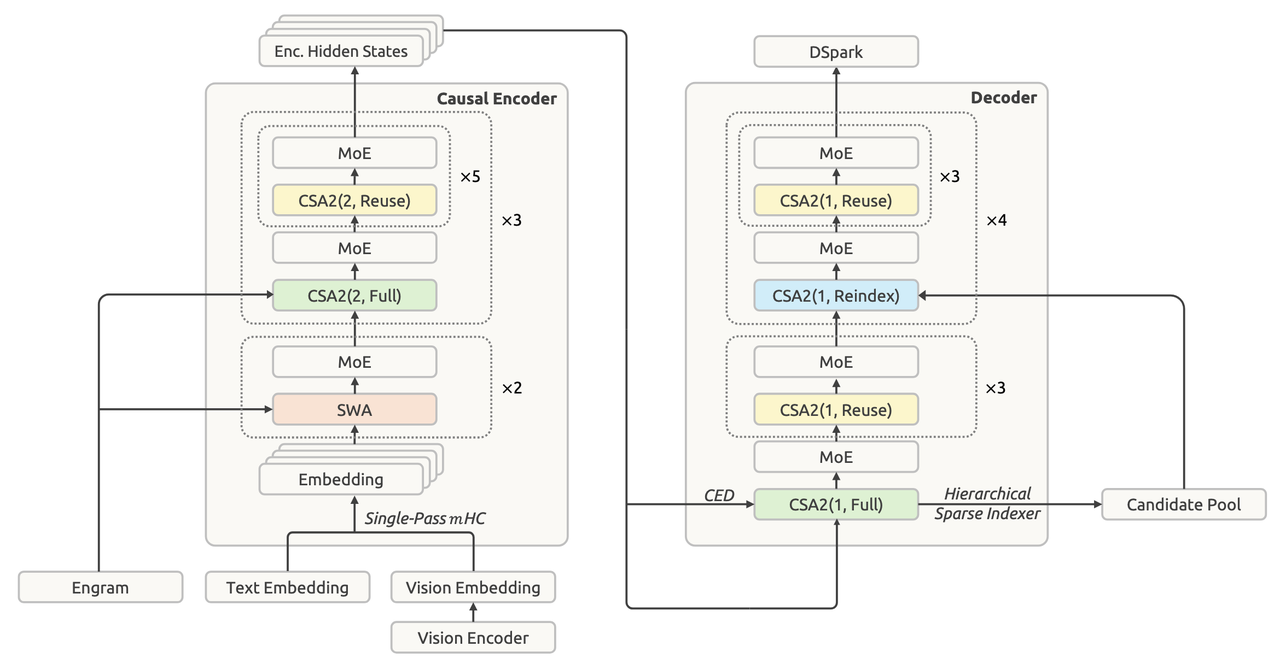
\includegraphics[width=0.98\linewidth,height=0.82\textheight,keepaspectratio]{images/DeepSeek-V4.1-Flash架构/fig-24.png}\end{center}

% source-block: 25 doxcnqCarSYLn8ZuhHO1GTZILnb text
\textcolor{feishuRed}{\textbf{上图是 DeepSeek-V4.1-Flash 架构}}，Attention 除了前 2 层的 SWA，其余层统一为 \incode{CSA2(ratio, mode)} ，\incode{ratio} 和 \incode{mode} 两个静态参数直接决定层性质，也是下面的关键内容：\incode{ratio} 来自 \incode{compress\_ratios}，\incode{mode} 由 \incode{kv\_source\_layer\_ids} 与 \incode{index\_source\_layer\_ids} 共同决定。\par

% source-block: 26 doxcn7j2oWyfU99EUknzMLoT5Eg text

% source-block: 27 doxcnDdwg4Ue3g0VsQBwaylbnGd heading2
\par\Needspace{8\baselineskip}\vspace{0.8em}\noindent \begin{tcolorbox}[boxrule=0pt,arc=3pt,colback=callRed,left=3pt,right=3pt,top=2pt,bottom=2pt,before skip=0pt,after skip=0pt]{\zihao{-2}\bfseries \textcolor{feishuBlue}{1.}\ CED（Causal Encoder-Decoder）：解码器全局 KV 由编码器最后一层投影}\end{tcolorbox}\par\vspace{0.28em}

% source-block: 28 doxcnd1Ilqhak45Mu8wy5ovnz41 text
\textcolor{feishuRed}{\textbf{动机：}} Agentic 场景工具调用频繁，每轮都产生新的 prefill 请求，KV cache miss 造成极高 TTFT。DeepSeek V4 的 prefill 复杂度是 $O(NL)$，$N$ 为序列长度、$L$ 为层数，在 Input-Heavy 负载下是主要成本。\par

% source-block: 29 doxcnMABc12y6bvthS6xadKbKVc text
\textcolor{feishuRed}{\textbf{实现：}} 做法类似\href{https://arxiv.org/pdf/2405.05254}{《You Only Cache Once: Decoder-Decoder Architectures for Language Models》}（YOCO）的策略，让模型后半层共享前半层 KV cache，DeepSeek V4.1-Flash 的 CED（Causal Encoder-Decoder） 在 YOCO 上做两处增强：\par
\begin{itemize}
\item 
% source-block: 30 doxcnsJmvXDSibDzrkz2BrkXqVc bullet
全局 KV 从 Encoder 输出投影：给每个解码器层配独立投影权重，从共享 hideen states 中独立投影。\par
\item 
% source-block: 31 doxcnRTTgGedS7YQ5huw4CEFdM3 bullet
保留逐层的局部注意力以维持局部 KV 的计算深度。\par
\end{itemize}

% source-block: 32 doxcnyhFwxAhjyyMWG5rq4trnHh heading3
\par\Needspace{8\baselineskip}\vspace{0.8em}\noindent \begin{tcolorbox}[boxrule=0pt,arc=3pt,colback=callOrange,left=3pt,right=3pt,top=2pt,bottom=2pt,before skip=0pt,after skip=0pt]{\zihao{3}\bfseries \textcolor{feishuBlue}{1.1}\ 全局 KV 从 Encoder 输出投影}\end{tcolorbox}\par\vspace{0.28em}

% source-block: 33 doxcnRPkKfKgp3jvGKmT3oOfUkE text
把 Transformer 的前 $L/2$ 层作为 Causal Encoder，对后 $L/2$ 层解码器，全局 KV 不由本层 hidden state $H_l$ 得到，而是从第 $L/2$ 层输出的 hidden state $H_{L/2}$ 直接投影：\par

% source-block: 34 doxcnRzt8we64uMRP0O6w5uoqN9 text
\bigmath{C_l=H_{L/2}W_l^{KV},\quad Z_l=H_{L/2}W_l^Z,\quad l>\frac L2}
\begin{itemize}
\item 
% source-block: 35 doxcniCBSymZTstu7QKdXwBcdVb bullet
$H_{L/2}\in\mathbb{R}^{N\times d}$ 是 Causal Encoder 最后一层的输出，$d$ 为隐藏维度（5120）。\par
\item 
% source-block: 36 doxcn74FVyWvY9zslBgGiGMEYob bullet
$C_l$ 是第 $l$ 层的 KV 条目，$Z_l$ 是对应的压缩权重。\par
\item 
% source-block: 37 doxcnfQWFmFiPVqs1mbT4hWotdh bullet
$W_l^{KV},W_l^Z$ 是层相关的投影权重，各解码器层拿到的仍是各自的 KV。\par
\end{itemize}

% source-block: 38 doxcnNzGFcZAs59cZ5rhx4wQLwb text
因此 Prefill 的 FLOPs 大约可以减半：在拿到 $H_{L/2}$ 之后，后 $L/2$ 层的全局 KV 通过两次矩阵乘补齐，不需要经过后 $L/2$ 层的完整计算（Attention、MoE 等）。\par

% source-block: 39 doxcnnqLvpaJAHRmSSOeeH5WIIe quote_container
\begin{feishuquote}

% source-block: 204 doxcnnO9E4jitaETF4W0EGOLASd text
关键注意点：虽然上面的公式（来自 DeepSeek V4.1 Flash 原论文）是每个解码器层都有自己的 $W_l^{KV}$，但是CSA2 的 Reuse 模式（下文会介绍）直接共享 Main KV，因此实际只实例化一份全局 KV，解码器层直接共享。\par
\end{feishuquote}

% source-block: 40 doxcnz68HkqkVCqSeRCfJe23a0d heading3
\par\Needspace{8\baselineskip}\vspace{0.8em}\noindent \begin{tcolorbox}[boxrule=0pt,arc=3pt,colback=callOrange,left=3pt,right=3pt,top=2pt,bottom=2pt,before skip=0pt,after skip=0pt]{\zihao{3}\bfseries \textcolor{feishuBlue}{1.2}\ Decoder SWA Bounded Replay}\end{tcolorbox}\par\vspace{0.28em}

% source-block: 41 doxcnNjdoLXyehiZCgma9nwgsKh text
DeepSeek-V4.1-Flash 的 CSA2 是由 \href{https://my.feishu.cn/wiki/UsuawakRYiqacxkD9vxcKzylnoe}{DeepSeek V4 的 CSA} 简化而来的，CSA 下文会介绍。CSA2 仍然保留了 Sliding Window Attention 的计算细节：\par

% source-block: 42 doxcnr6Q7HNx8o4XmP16Tm480yg callout
\begin{feishubox}{callGreen}{📌}

% source-block: 205 doxcnL6UuR8M1IxR1b6qSMmjixj text
每层保留 \incode{n\_win=128} 个 uncompressed KV，跟压缩 KV 拼在一起做 attention：\par

% source-block: 206 doxcnRdn03vV9BedjtoF4BPmwhe text
\textbf{这其实是对 CSA/HCA 的漏洞修复，有两个动机：}\par
\begin{enumerate}
\item 
% source-block: 207 doxcn1LE3GUi7Fo0ujoiy6wKUTf ordered
维持严格因果性带来的块内盲区：CSA/HCA 的 query 只能 select "已经完成的"压缩块，跟query 同属一个压缩块的 m-1 个邻居彼此看不见（CSA 的 m=4、HCA 的 m'=128 都有这个问题）。\par
\item 
% source-block: 208 doxcnNt5z6rTjjXPRFGmsyc7dGg ordered
最近邻优先：最近 token相关性最强，留未压缩的精确版本比压缩后的更精确。\par
\end{enumerate}
\end{feishubox}

% source-block: 43 doxcnyBA2RYtDMD8yp5mYFZe7Gb text
而局部注意力 SWA 的逻辑不是上面的共享全局 KV，SWA 的 key 与 value 都从本层的 $H_l$ 直接计算，但是代价就是 prefill 阶段解码器仍需多处理 $n_{\mathrm{win}}\times L/2$ 个 Token（$L/2$层，每层状态最多向前拓展$n_{\mathrm{win}}$个 Token）才能补齐完整的 SWA 状态，多轮短提示词场景下这笔开销不可忽略。\par

% source-block: 44 doxcnzhlrqLM3GMtXw2L3DtR1Fg text
但是 DeepSeek V4.1 Flash 消融观察到 SWA 的实际有效感受野远小于理论上的 $n_{\mathrm{win}}\times L/2$，并且模型退化可以忽略，因此 V4.1 Flash 据此提出 Decoder SWA Bounded Replay：只重放提示词最后 $n_{\mathrm{win}}$ 个 token 做近似重建，因此$N\gg n_{\mathrm{win}}$ 时 prefill 复杂度从 $O(NL)$ 降到 $O(NL/2+n_{\mathrm{win}}\times L/2)\approx O(NL/2)$。\par

% source-block: 45 doxcn3KOTz2XlF1U7hIJyaS3gIc text

% source-block: 46 doxcnrcxV5QXZtnuWhn5AYCE8Oh heading2
\par\Needspace{8\baselineskip}\vspace{0.8em}\noindent \begin{tcolorbox}[boxrule=0pt,arc=3pt,colback=callRed,left=3pt,right=3pt,top=2pt,bottom=2pt,before skip=0pt,after skip=0pt]{\zihao{-2}\bfseries \textcolor{feishuBlue}{2.}\ CSA2（Compressed Sparse Attention 2）}\end{tcolorbox}\par\vspace{0.28em}

% source-block: 47 doxcnTwMO4HQVNcg2Pa6mID089f heading3
\par\Needspace{8\baselineskip}\vspace{0.8em}\noindent \begin{tcolorbox}[boxrule=0pt,arc=3pt,colback=callOrange,left=3pt,right=3pt,top=2pt,bottom=2pt,before skip=0pt,after skip=0pt]{\zihao{3}\bfseries \textcolor{feishuBlue}{2.1}\ 回顾第一代 CSA（Compressed Sparse Attention）}\end{tcolorbox}\par\vspace{0.28em}

% source-block: 48 doxcndmb9uzFvQ09LXwHIngu2s6 text
首先简要回顾 \href{https://my.feishu.cn/wiki/UsuawakRYiqacxkD9vxcKzylnoe}{DeepSeek-V4 架构：技术报告/源码解析}中 CSA 的架构：\par

% source-block: 49 doxcnRI6nMZiZ0MJujMpF9tN1pB grid
\begin{tcbraster}[raster columns=2,raster equal height=rows,raster column skip=8pt,raster row skip=8pt,raster left skip=0pt,raster right skip=0pt]

% source-block: 209 doxcnH67hmRA7ofEWZrPEvrCP6q grid_column
\begin{tcolorbox}[enhanced,boxrule=0pt,colback=white,colframe=white,left=0pt,right=0pt,top=0pt,bottom=0pt]
% source-block: 210 doxcndyR7kZKUBWFiDXlwtLhwVb image
\begin{center}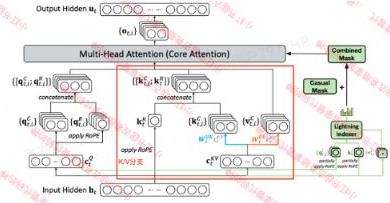
\includegraphics[width=0.98\linewidth,height=0.82\textheight,keepaspectratio]{images/DeepSeek-V4.1-Flash架构/fig-210.png}\par DS V3.2 的 DSA\end{center}
\end{tcolorbox}
% source-block: 211 doxcnxuRRYTgMlRYimIiRUjYR9Z grid_column
\begin{tcolorbox}[enhanced,boxrule=0pt,colback=white,colframe=white,left=0pt,right=0pt,top=0pt,bottom=0pt]
% source-block: 212 doxcnWuKaQVVjuIveYd3bjcsTtd image
\begin{center}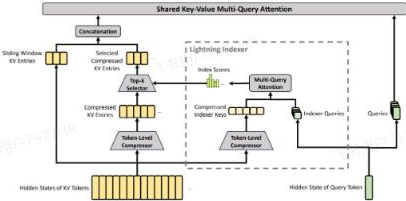
\includegraphics[width=0.98\linewidth,height=0.82\textheight,keepaspectratio]{images/DeepSeek-V4.1-Flash架构/fig-212.png}\par DS V4 的 Compressed Sparse Attention\end{center}
\end{tcolorbox}
\end{tcbraster}

% source-block: 50 doxcnat19UTeAGI0NKFr3aTfYny text
\textcolor{feishuRed}{DeepSeek V3.2 的 DSA 直接在原始 KV 上用 Lightning Indexer 做 top-K Selection，每个 query 的 KV 候选大小仍是 }$O(n)$\textcolor{feishuRed}{。V4 先进行 KV Sparse 压缩到 }$O(n/m)$\textcolor{feishuRed}{ 再进行 Selection，因此 indexer 排序候选集变为之前的 }$1/m$\textcolor{feishuRed}{。分两步实现，先 KV Compress 把}$O(n)$\textcolor{feishuRed}{序列压缩到}$O(n/m)$\textcolor{feishuRed}{，后 Lightning Indexer 进行 Top-K 选择。}\par

% source-block: 51 doxcnBOYUDtfCNgt3eNxdQbvidh heading5
\par\Needspace{8\baselineskip}\vspace{0.8em}\noindent {\zihao{4}\bfseries \textcolor{feishuRed}{\textbf{KV Compress}}}\par\vspace{0.28em}

% source-block: 52 doxcnpREOvA6c43zeBzDOxxXm7b text
输入 $H\in\mathbb{R}^{n\times d}$，首先用两个可学习的 KV projection $W_a^{KV},W_b^{KV}\in\mathbb{R}^{d\times c}$映射到 Latent（这里和 MLA 的逻辑是一样的），但是需要注意这里映射了 2 个 Latent 表示为的是压缩的时候进行窗口平滑（Sliding Window）：\par

% source-block: 53 doxcndwUzMXgBHZWm6eRw5SEDuh text
\bigmath{C^a=H\cdot W_a^{KV},C^b=H\cdot W_b^{KV}}

% source-block: 54 doxcnM5eKFav0pRyApdhnrzxGQd text
此外，需要对应的另外两个可学习的 KV projection $W_a^Z,W_b^Z\in\mathbb{R}^{d\times c}$映射另外一组 Gate Latent，映射维度和上面一样，用来计算压缩时候的加权率（Gating）：\par

% source-block: 55 doxcnFb6L9IC5589swn6IAbrSkc text
\bigmath{Z^a=H\cdot W_a^Z,Z^b=H\cdot W_b^Z}

% source-block: 56 doxcnuLSt7psyzcolpKmQnEpOVW text
然后 $m$ 个连续 token 计算两个压缩加权比率（\textcolor{feishuRed}{论文里面取 }$m=4$）：\par

% source-block: 57 doxcnFiN2cRCsKJgNCN2TvJw9Rf text
\bigmath{\begin{aligned}&[S^a_{mi:m(i+1)-1};S^b_{m(i-1):mi-1}]\\&\quad=\mathrm{Softmax}_{\mathrm{row}}\!\left([Z^a_{mi:m(i+1)-1}+B^a;\ Z^b_{m(i-1):mi-1}+B^b]\right)\end{aligned}}

% source-block: 58 doxcnLDRX7ZmC1kLWW5k1fSrdKf text
用上面的加权比率就可以将 $m$ 个连续 token 合成一个 compressed entry $C_i^{\mathrm{Comp}}$，注意 $C^a$ 用当前窗口 $[mi,m(i+1)-1]$，$C^b$ 用\textbf{前一个}窗口 $[m(i-1),mi-1]$，\textcolor{feishuRed}{两个窗口叠加，这是 CSA 平滑的关键}：\par

% source-block: 59 doxcn6dGs60lG6UtA5fKTMv0Jab text
\bigmath{C_i^{\mathrm{Comp}}=\sum_{j=mi}^{m(i+1)-1}S_j^a\odot C_j^a+\sum_{j=m(i-1)}^{mi-1}S_j^b\odot C_j^b}
\begin{itemize}
\item 
% source-block: 60 doxcnYHZ1nXX941RNNsdvr9iIY9 bullet
$B^a,B^b\in\mathbb{R}^{m\times c}$：可学习的位置偏置（\textcolor{feishuRed}{相当于滑动窗口的 Absolute Position Embedding}）。\par
\item 
% source-block: 61 doxcndoe0DtRhaPs8dnSb2sknUc bullet
$\odot$：Hadamard 积，即对应位置相乘，结果 shape 不变。\par
\end{itemize}

% source-block: 62 doxcneyUDiZ0yilWIEoUthfbv9g heading5
\par\Needspace{8\baselineskip}\vspace{0.8em}\noindent {\zihao{4}\bfseries \textcolor{feishuRed}{\textbf{Lightning Indexer}}}\par\vspace{0.28em}

% source-block: 63 doxcnIZvCFR9aveVktuhTLasLfc text
对 query token $t$，先生成低秩 Latent 再生成 indexer queries（本质上仍然是 MLA）：\par

% source-block: 64 doxcntui96BVdsJw25ilD8GgZpc text
\bigmath{\mathbf c_t^Q=\mathbf h_tW^{DQ}}

% source-block: 65 doxcn7IG09VmVHafenxLRgxYBKb text
\bigmath{[\mathbf q_{t,1}^I;\ldots;\mathbf q_{t,n_h^I}^I]=\mathbf q_t^I=\mathbf c_t^QW^{IUQ}}

% source-block: 66 doxcnJvnKCSc4sSFpCZV2L6gn1e text
同时需要生成 query head 之间的加权权重（$n_h^I$ 表示 Indexer 的 query 的 head 数量）：\par

% source-block: 67 doxcnqjPEqy6UQjHzV1swnlFiXc text
\bigmath{[w_{t,1}^I;w_{t,2}^I;\ldots;w_{t,n_h^I}^I]=\mathbf w_t^I=\mathbf h_t\cdot W^w,}

% source-block: 68 doxcnYGqt6hhoOGUJKEs2PTqsIe text
然后应用 ReLU 风格的 index score（需要在多 head 之间求和）：\par

% source-block: 69 doxcnTaRTGZ1jhU3nIkKoR8NVDf text
\bigmath{I_{t,s}=\sum_{h=1}^{n_h^I}w_{t,h}^I\cdot\mathrm{ReLU}(\mathbf q_{t,h}^I\cdot K_s^{\mathrm{IComp}})}

% source-block: 70 doxcnNsSMexcTLHX7MKXHFkYWzh text
Top-k 选择：$C_t^{\text{SprsComp }}=\left\{C_s^{\text{Comp }}\mid I_{t,s}\in\mathrm{Top}\mathord{-}\mathrm{k}(I_{t,:})\right\}$。\par

% source-block: 71 doxcnQBzGD4rGDQdT0UJr1CoVdf heading5
\par\Needspace{8\baselineskip}\vspace{0.8em}\noindent {\zihao{4}\bfseries \textcolor{feishuRed}{\textbf{Shared KV MQA }}}\par\vspace{0.28em}

% source-block: 72 doxcnUspU3uPBrZ0ebxCz4X9SX7 text
选出 top-k compressed entries 之后做 MQA：\par

% source-block: 73 doxcn9j6C1Gbj1KPOSgouJWwTqg text
\bigmath{[\mathbf q_{t,1};\ldots;\mathbf q_{t,n_h}]=\mathbf q_t=\mathbf c_t^QW^{UQ}}

% source-block: 74 doxcndXMXhAxEdgGgAcwFyg9agI text
\bigmath{\begin{aligned}\mathbf o_{t,i}=\mathrm{CoreAttn}(&\mathrm{query}=\mathbf q_{t,i},\\ &\mathrm{key}=C_t^{\mathrm{SprsComp}},\ \mathrm{value}=C_t^{\mathrm{SprsComp}})\end{aligned}}

% source-block: 75 doxcn3m4VXZJnMQdZYFSbiG9laf text
最后把多个 head 的 $\mathbf o_{t,i}$ 拼起来得到 $\mathbf o_t=[\mathbf o_{t,1};\mathbf o_{t,2};\ldots;\mathbf o_{t,n_h}]\in\mathbb{R}^{cn_h}$。\par

% source-block: 76 doxcn6tXyWkVYJdOplOzBC3KRfc heading5
\par\Needspace{8\baselineskip}\vspace{0.8em}\noindent {\zihao{4}\bfseries \textcolor{feishuRed}{\textbf{Grouped Output Projection}}}\par\vspace{0.28em}

% source-block: 77 doxcnTig2NMue9kXDBfvBePo1Vc text
上一步合并的 $\mathbf o_t$的 hidden dim $cn_h$ 非常大，如果直接进行 $w_o$投影，投影矩阵是 $cn_h\times d$，参数量和计算量都很夸张。因此先分组降维，再合并投影。\par
\begin{itemize}
\item 
% source-block: 78 doxcn6R25qTBZGqkCzwsoEvNc8g bullet
\textbf{分组：}把 $n_h$ 个头平均分成 $g$ 组,每组有 $n_h/g$ 个头。每组拼起来的向量是: $\mathbf o_{t,i}^G\in\mathbb R^{c\cdot n_h/g}$\par
\item 
% source-block: 79 doxcnBSzRxzMAJSnucKYIrhGodd bullet
\textbf{组内降维：}每一组各自用一个小的投影矩阵,把 $c\cdot n_h/g$ 维压到 $d_g$ 维:$\mathbf o_{t,i}^GW_g^{\mathrm{o\_a}}=\mathbf o_{t,i}^{G^{\prime}}\in\mathbb R^{d_g}$\par
\item 
% source-block: 80 doxcnWjcsKYZAL7vxGaZZ5uI6Vg bullet
\textbf{合并后再投影到 }$d$\textbf{：}把 $g$ 个降维后的小向量拼起来(总共 $d_g\cdot g$ 维),再用一个投影矩阵送到最终的 $d$ 维: $\mathbf o_{t,i}^{G^{\prime}}=\widehat{\mathbf o}_tW^{\mathrm{o\_b}}\in\mathbb R^d$\par
\end{itemize}

% source-block: 81 doxcnSElyvsI82bYTrTm6LnEvzc text

% source-block: 82 doxcn0XNQFH1WxqKtYmdsxRBwYe heading3
\par\Needspace{8\baselineskip}\vspace{0.8em}\noindent \begin{tcolorbox}[boxrule=0pt,arc=3pt,colback=callOrange,left=3pt,right=3pt,top=2pt,bottom=2pt,before skip=0pt,after skip=0pt]{\zihao{3}\bfseries \textcolor{feishuBlue}{2.2}\ CSA2 相比 CSA 进行简化}\end{tcolorbox}\par\vspace{0.28em}

% source-block: 83 doxcndxElg9vzi9bUgAitd3pHsd text
\textcolor{feishuRed}{\textbf{动机：}} DeepSeek V4 的第一代 CSA 的设计推高了实现复杂度与训练开销：\par
\begin{itemize}
\item 
% source-block: 84 doxcnt2zY1chF3mBBo1I6vs86pf bullet
在压缩率 $m$ 设置下，每条 main KV 由 $2m$ 条原始 KV 生成，即 $C^a=H\cdot W_a^{KV}, C^b=H\cdot W_b^{KV}$。\par
\item 
% source-block: 85 doxcnKx7fnxXa3Okl4qoCtFgMTg bullet
压缩时带可学习的绝对位置偏置 $B^a,B^b$，用来编码这 $2m$ 个位置。\par
\item 
% source-block: 86 doxcnb4wp3pQvKlR2IMlf7JXbdb bullet
indexer 的 Key 从 hidden state 独立压缩。\par
\end{itemize}

% source-block: 87 doxcnuB6efUKfs9IL4hhhTF0Hme text
\textcolor{feishuRed}{\textbf{实现：}} CSA2 采用更简单的 KV 压缩建模，直接退化成单个窗口内的 softmax 池化：\par

% source-block: 88 doxcnF2ffUt6iksU2RvfmP8SjUc text
\bigmath{C=HW^{KV},Z=HW^Z}

% source-block: 89 doxcnaRVqiXuKag6L1Q82Fzh4pc text
\bigmath{\begin{aligned}S_{mi:m(i+1)-1}&=\mathrm{Softmax}_{\mathrm{row}}\!\left(Z_{mi:m(i+1)-1}\right),\\ C_i^{\mathrm{Comp}}&=\mathrm{RMSNorm}\!\left(\sum_{j=mi}^{m(i+1)-1}S_j\odot C_j\right)\end{aligned}}
\begin{itemize}
\item 
% source-block: 90 doxcnOEXTBl1AJrgOKQLeL2rZue bullet
$H\in\mathbb{R}^{N\times d}$ 是当前层输入，解码器层为 $H_{L/2}$。\par
\item 
% source-block: 91 doxcnVJjV1AWUgtaJkqGK1jgUsc bullet
$C_i^{\mathrm{Comp}}$ 是第 $i$ 条压缩 KV 条目，序列长度是原本的 $1/m$。\par
\end{itemize}

% source-block: 92 doxcnZ4ow2C03qj1YRbgVWeZK2c text
对照 \href{https://my.feishu.cn/wiki/UsuawakRYiqacxkD9vxcKzylnoe}{DeepSeek-V4 架构：技术报告/源码解析}\textbf{ }里 CSA 的同一组公式，关键差别在于取消了可学习的绝对位置偏置 $B^a$、$B^b$ 与错位叠加，增加了一个 RMSNorm。对应到实现代码 \incode{Compressor.forward}：\par

% source-block: 93 doxcn01dB4vfK3Gk2gW3zWS1s4d code
% Code block omitted at user request.

% source-block: 94 doxcnUsgE8w4WRrDd6my2MBd7md text
对于 indexer K 的简化：CSA2 直接把 main KV 条目投影成 indexer K，$K_s^I=\mathrm{RMSNorm}(C_s^{\mathrm{Comp}}W^{IK})$，不再单独从 hidden state 压缩：\par

% source-block: 95 doxcnVSzfqNS4enbJAEAzhgVhvd code
% Code block omitted at user request.

% source-block: 96 doxcn28okUNsxYnrdKTwjXoYBaf text
Indexer 打分的形式和 DeepSeek V4 一致，即 ReLU 风格的 index score：\par

% source-block: 97 doxcnCtzDLGexHbBLGuK61mMdTe text
\bigmath{I_{t,s}=\sum_h w_{t,h}^I\cdot\mathrm{ReLU}(\mathbf{q}_{t,h}^I\cdot K_s^I)}

% source-block: 98 doxcnsOUYWHq1hlq16UZECHqDGb quote_container
\begin{feishuquote}

% source-block: 213 doxcn2CcdsbSc2OaueE8KN1414b text
\href{https://scnajei2ds6y.feishu.cn/wiki/KOBowKTbgiv6ewkHhEBc6qCNnPe}{GLM-5.3-Flash} 同样也是用了同一机制。\par
\end{feishuquote}

% source-block: 99 doxcnQcpM1foBi6yqqB7u4tCjHd text
但是相比 DeepSeek V4 缩放常数不同：V4 是 $(d_h^I)^{-1/2}$，V4.1 是 $(d_h^I)^{-1/2}(n_h^I)^{-1/2}$，分摊 head 数对分数的影响。\par

% source-block: 100 doxcnSzq1KQQDTfDzg5PC4JfScd text

% source-block: 101 doxcnRxzJ03I2MSchKYv3AzHeYc heading3
\par\Needspace{8\baselineskip}\vspace{0.8em}\noindent \begin{tcolorbox}[boxrule=0pt,arc=3pt,colback=callOrange,left=3pt,right=3pt,top=2pt,bottom=2pt,before skip=0pt,after skip=0pt]{\zihao{3}\bfseries \textcolor{feishuBlue}{2.3}\ CSA2 的 Full / Reindex / Reuse 模式}\end{tcolorbox}\par\vspace{0.28em}

% source-block: 102 doxcnBpjapGO1N0AK25euLO659e text
CSA2 层可以被设置成 Full / Reindex / Reuse 三种静态模式。Full / Reindex / Reuse 三种静态模式共有的部分是 main Q 和自己的 SWA KV，区别在于 main KV、indexer K、Top-K Indeices 的来源。\par

% source-block: 103 doxcnA9CWEoYqRpGUdnA6jGsyWg image
\begin{center}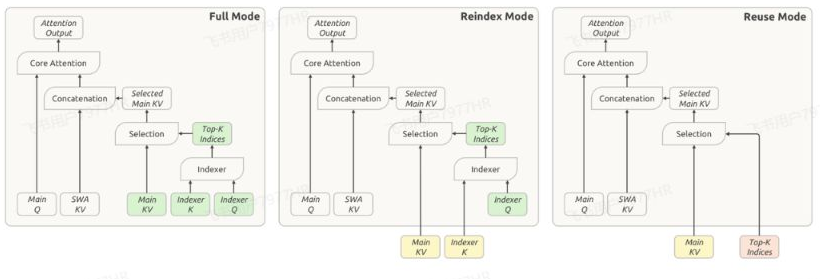
\includegraphics[width=0.98\linewidth,height=0.82\textheight,keepaspectratio]{images/DeepSeek-V4.1-Flash架构/fig-103.png}\end{center}
\begin{itemize}
\item 
% source-block: 104 doxcn5RGfKtgwaCl7Yu5PRc809g bullet
\textcolor{feishuRed}{\textbf{Full}}：即默认的 CSA 计算模式，main KV、indexer K、Top-K Indeices 均由当前层重新计算，即压缩 main KV、投影 indexer K、执行 indexer 得到新的 Top-K Indeices。\par
\item 
% source-block: 105 doxcnrMs9sH8ObGlbBOU1GqJt7f bullet
\textcolor{feishuRed}{\textbf{Reindex}}：main KV 与 indexer K 复用最近一个 Full 层，但用本层的 indexer Q 重新打分选出当前层的 Top-K Indeices，稀疏选择因此能逐层变化并且保持 cache 共享。\par
\item 
% source-block: 106 doxcnxuFQQ41tuGdgTj5QMKFd9g bullet
\textcolor{feishuRed}{\textbf{Reuse}}：main KV 与 Top-K indexer 都复用，因此不必计算 indexer Q / indexer K。\par
\end{itemize}

% source-block: 107 doxcn454Vbpz0JemVJM3jDumYhg text
在 1M 量级的长文本注意力下，两个关键的开销是\incode{计算}和\incode{缓存}，共享 main KV 与 indexer K 目标是缓解 cache 存储压力，复用 Top-K 缓解的是 indexer 计算压力。Reindex 是\incode{计算}和\incode{缓存}平衡的中间，保住存储共享的同时保留层间 Top-K 选择差异，Reuse 则类似 \href{https://my.feishu.cn/wiki/CGgqwKi1tihc3JkQby9cx2gDnFb}{GLM-5.2} 的 IndexShare，跨层复用稀疏选择。\par

% source-block: 108 doxcnGIQjVwN7BcJE94kJKqm66c text

% source-block: 109 doxcnfi0fKFz2QOdtsq5lVnJeye heading3
\par\Needspace{8\baselineskip}\vspace{0.8em}\noindent \begin{tcolorbox}[boxrule=0pt,arc=3pt,colback=callOrange,left=3pt,right=3pt,top=2pt,bottom=2pt,before skip=0pt,after skip=0pt]{\zihao{3}\bfseries \textcolor{feishuBlue}{2.4}\ 层级调度：从 kv\_source 与 index\_source 列表推导}\end{tcolorbox}\par\vspace{0.28em}

% source-block: 110 doxcnqicKxV1bL1OnZB0ODhMFnc grid
\begin{tcbraster}[raster columns=2,raster equal height=rows,raster column skip=8pt,raster row skip=8pt,raster left skip=0pt,raster right skip=0pt]

% source-block: 214 doxcnixQSBZGsU2xwNCpMuPtpIg grid_column
\begin{tcolorbox}[enhanced,boxrule=0pt,colback=white,colframe=white,left=0pt,right=0pt,top=0pt,bottom=0pt]
% source-block: 215 doxcnwEZdINcB0pTSPpe67SToEd image
\begin{center}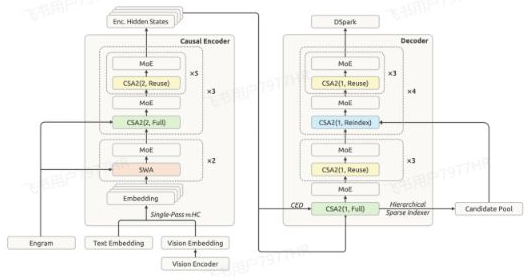
\includegraphics[width=0.98\linewidth,height=0.82\textheight,keepaspectratio]{images/DeepSeek-V4.1-Flash架构/fig-215.png}\end{center}
\end{tcolorbox}
% source-block: 216 doxcn9wBlshtyT4RsId0GmYriDf grid_column
\begin{tcolorbox}[enhanced,boxrule=0pt,colback=white,colframe=white,left=0pt,right=0pt,top=0pt,bottom=0pt]
% source-block: 217 doxcnScwBm34tjpfqg4iqSBoH4d image
\begin{center}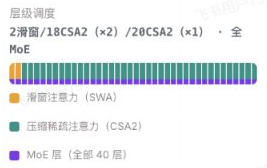
\includegraphics[width=0.98\linewidth,height=0.82\textheight,keepaspectratio]{images/DeepSeek-V4.1-Flash架构/fig-217.png}\end{center}
% source-block: 218 doxcnS51qGU0SqbrXB5bAubnNAh text
\end{tcolorbox}
\end{tcbraster}

% source-block: 111 doxcnqHvX0AstOsasOgzkTBZA9o text
DeepSeek-V4.1-Flash 的层级调度（右上图）是非常干净的 CSA2（除了前两层是 SWA），相比于 \href{https://my.feishu.cn/wiki/Gg57wvxiriwum6kVSlkctRy0nRh}{DeepSeek V4} 的 1:1 CSA + HCA 混合注意力看起来统一了很多，但是实质上 DeepSeek-V4.1-Flash 是通过两个维度去控制层注意力的模型，即上文 CSA2 的压缩率 $m$以及 Full / Reindex / Reuse 模式，参考左上图，\incode{CSA2（\_，\_）}的两个静态参数决定层的模式，层模式在 config.json 里没有显式字段，靠两个列表交叉判定：\par

% source-block: 112 doxcnpFyE9qBMg2Ufe47KqkMkl1 code
% Code block omitted at user request.

% source-block: 113 doxcnGSUGkBkXwaSQdXGmHpFhDh text
\textbf{层模式判断依据：}既是 KV 源又是 index 源的设置为 Full，只是 index 源的设置 Reindex，两者都不是设置 Reuse。\par

% source-block: 114 doxcnuzuFeKihwoYNacT3rdZa8c table
\begin{longtable}{|>{\raggedright\arraybackslash}p{3.28cm}|>{\raggedright\arraybackslash}p{3.28cm}|>{\raggedright\arraybackslash}p{3.28cm}|>{\raggedright\arraybackslash}p{3.28cm}|}\hline
\rowcolor{tableHead} 
% source-block: 220 doxcnQn58yjEkGyA3DT9cQ6zVmf text
架构层位置\par
 & 
% source-block: 222 doxcnYFwZ0UmKq6Z67wHao1PEfe text
层号\par
 & 
% source-block: 224 doxcn6bcxTNm1IqwP2S0Oo7fcIx text
压缩率（\incode{ratio}）\par
 & 
% source-block: 226 doxcnTtLaADTRIus5aUrdL8PznY text
模式（\incode{mode}）\par
 \\ \hline
\endfirsthead
\hline\rowcolor{tableHead} 
% source-block: 220 doxcnQn58yjEkGyA3DT9cQ6zVmf text
架构层位置\par
 & 
% source-block: 222 doxcnYFwZ0UmKq6Z67wHao1PEfe text
层号\par
 & 
% source-block: 224 doxcn6bcxTNm1IqwP2S0Oo7fcIx text
压缩率（\incode{ratio}）\par
 & 
% source-block: 226 doxcnTtLaADTRIus5aUrdL8PznY text
模式（\incode{mode}）\par
 \\ \hline
\endhead

% source-block: 228 doxcnfEAVXwvFWnUJrOLPusMC1e text
Encoder 前两层\par
 & 
% source-block: 230 doxcn5A1kHw9fLludMig6hbqLBb text
0, 1\par
 & 
% source-block: 232 doxcnfc31995C3u2db5txiFYTFd text
0\par
 & 
% source-block: 234 doxcnqg3g1bEUiSJrSlkMS1VJ3f text
SWA\par
 \\ \hline

% source-block: 236 doxcnPYXuOmOK4hzcobYulbKzqc text
Encoder 2 / 8 / 14 层\par
 & 
% source-block: 238 doxcndHRc9nXJAnDDAWSOkP3blf text
2 / 8 / 14\par
 & 
% source-block: 240 doxcnk0G3wgVywW08ol1fBs9RGh text
2\par
 & 
% source-block: 242 doxcnqSfFDq30QHivR8jhCnIrTb text
Full\par
 \\ \hline

% source-block: 244 doxcnQgH8tVcPBooKOz1YFU1OFc text
Encoder 其余\par
 & 
% source-block: 246 doxcnXQn8M8JjAESE5V9yZyZSFc text
总计 15 层\par
 & 
% source-block: 248 doxcnD0LkH8Zqo8oQoqK2mLLRtd text
2\par
 & 
% source-block: 250 doxcnNxFJQal8Mcqq1vePuqeHjd text
Reuse\par
 \\ \hline

% source-block: 252 doxcn4OcbQ2BaVxQ7y72U3Qm8if text
Decoder 第一层\par
 & 
% source-block: 254 doxcnGaWeRdhrfPf08LeHHmOaig text
20\par
 & 
% source-block: 256 doxcnANf03vwDsUTWMgDijRFrIh text
1\par
 & 
% source-block: 258 doxcnUgcQU2ifIr8b9IfI0LiKub text
Full\par
 \\ \hline

% source-block: 260 doxcnvvQDQ4BATPIM4hYjxg5jVb text
Decoder 21 / 22 / 23 层\par
 & 
% source-block: 262 doxcnMVCxAr0MYZc0QBvvRP7V0d text
21 / 22 / 23\par
 & 
% source-block: 264 doxcnATXChxoeLl5N7CL25F2eoP text
1\par
 & 
% source-block: 266 doxcn3cPDmtDiQmjyzsc2itLgdh text
Reuse\par
 \\ \hline

% source-block: 268 doxcnjxRrFSRBeWGY9h8LO8yO1c text
Decoder 24 / 28 / 32 / 36 层\par
 & 
% source-block: 270 doxcnxDuXpjofLwkXOPdd67KC9d text
24 / 28 / 32 / 36\par
 & 
% source-block: 272 doxcnlA9uPYAK9Bnd2WAjiASdRf text
1\par
 & 
% source-block: 274 doxcnKMEHC65BzsUdQZRVva2fQU text
Reindex\par
 \\ \hline

% source-block: 276 doxcnE2w9KXC4qtD0nl3CkZklYf text
Decoder 其余\par
 & 
% source-block: 278 doxcnk04BVA8P0fD0CkEPbSkNLg text
总计 12 层\par
 & 
% source-block: 280 doxcnvSd3BVVqwbwDaoXx2ndOfg text
1\par
 & 
% source-block: 282 doxcn4RrhanhlDwF9qrUe2SBord text
Reuse\par
 \\ \hline
\end{longtable}

% source-block: 115 doxcn4a5agaXhJyn5hOwNAElGpa text

% source-block: 116 doxcntba2J5iLgvcFGEtSib1TSf heading3
\par\Needspace{8\baselineskip}\vspace{0.8em}\noindent \begin{tcolorbox}[boxrule=0pt,arc=3pt,colback=callOrange,left=3pt,right=3pt,top=2pt,bottom=2pt,before skip=0pt,after skip=0pt]{\zihao{3}\bfseries \textcolor{feishuBlue}{2.5}\ Hierarchical Sparse Indexer}\end{tcolorbox}\par\vspace{0.28em}

% source-block: 117 doxcnBKYUCMkw0sYcNr4F773Ieg text
\textcolor{feishuRed}{\textbf{动机：}} 跨层索引复用（CSA2 的 Reuse）减少了 indexer 的执行次数，但剩下的其他层的 Indexer 仍要对全部因果可见位置打分，计算压力随上下文线性增长，在 1M 上下文时重新变成主要瓶颈。\par

% source-block: 118 doxcnYPJHQzF7aX2cxkc1epRGnd text
\textcolor{feishuRed}{\textbf{实现：}} 解码器第一个 Full 层（第 20 层）除给选择当前层 Top-K，还额外做一次块级选择：每块取块内位置的最高 index score 作为这个块的分数，选出分数最高的若干块，这些块覆盖的位置作为候选池供后面的 Reindex 层复用。\par

% source-block: 119 doxcnyyUHmznzZ4Us96DbY6QOpg image
\begin{center}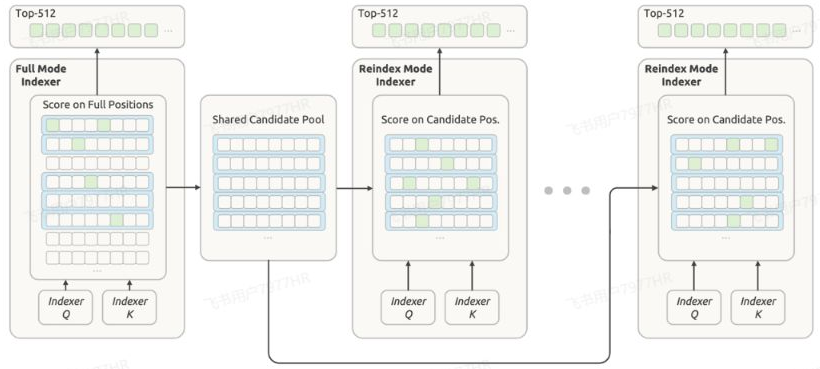
\includegraphics[width=0.98\linewidth,height=0.82\textheight,keepaspectratio]{images/DeepSeek-V4.1-Flash架构/fig-119.png}\end{center}

% source-block: 120 doxcnJAL7fFfP1cRgQOzf73ckph text
这个过程可以很直观的被上面的图示表示，公式可以表述为：\par

% source-block: 121 doxcnOyBkID3i4QMHuz4z4Ik6Of text
\bigmath{\widetilde I_{t,b}=\max_{s\in b}I_{t,s},\quad\mathcal B_t=\mathrm{Top}\text{-}k_{\mathrm{blk}}\!\left(\widetilde I_{t,:}\right)}
\begin{itemize}
\item 
% source-block: 122 doxcnhL2iSXTlWXdRUhqigtVVPe bullet
$b$ 是块索引，$\widetilde I_{t,b}$ 是查询 $t$ 对块 $b$ 的分数。\par
\item 
% source-block: 123 doxcnS9EeV5QV2XOVis3ajtw1Xe bullet
$\mathcal B_t$ 是选中的块集合，Top-K 大小为 \incode{candidate\_topk\_blocks}。\par
\end{itemize}

% source-block: 124 doxcnaac2qj2wq981j5onHcBj2f text
因此，Hierarchical Sparse Indexer 把深层 indexer 的每 query 打分量限制在一个固定上限内，降低了计算量：\par

% source-block: 125 doxcnUPBGzqxtgrv0AFe1AUkVed code
% Code block omitted at user request.

% source-block: 126 doxcnks67mSD6ZaLQlm78efjGue quote_container
\begin{feishuquote}

% source-block: 283 doxcn8Th2IodY9WtbCUC2t9bEkd text
关键细节：\par
\begin{itemize}
\item 
% source-block: 284 doxcnLrPTvkHAxGMmEJXwStrPfb bullet
最新的块还没被填充完，被显式设置$+\infty$ 强制保留。\par
\item 
% source-block: 285 doxcnkZq5ouRrnq7CTN7T4lmUdb bullet
Hierarchical Sparse Indexer 在后训练阶段引入，因此训推不一致的问题被后训练缓解。\par
\end{itemize}
\end{feishuquote}

% source-block: 127 doxcnXlZ6vo6JhcY3qTDrRMpuvc text
Hierarchical Sparse Indexer 带来的问题：\par
\begin{itemize}
\item 
% source-block: 128 doxcnoxuP2YMCOltA9ESFHGppAJ bullet
第 20 层（Decoder 第一个 Full 层）仍要全范围扫描。\par
\item 
% source-block: 129 doxcn4fgudPyezCw9KtK6oQlcsh bullet
候选池由第 20 层（Full）单独决定，深层 Selection 被这一层的判断限制，可能带来退化。\par
\end{itemize}

% source-block: 130 doxcna4BQKWwJmQq0KaoN0Q1ane text

% source-block: 131 doxcnrAKAcqCanyCaUWroo4Hnlf heading2
\par\Needspace{8\baselineskip}\vspace{0.8em}\noindent \begin{tcolorbox}[boxrule=0pt,arc=3pt,colback=callRed,left=3pt,right=3pt,top=2pt,bottom=2pt,before skip=0pt,after skip=0pt]{\zihao{-2}\bfseries \textcolor{feishuBlue}{3.}\ Engram}\end{tcolorbox}\par\vspace{0.28em}

% source-block: 132 doxcnmX9XTfImqGq7rgrhfZaoRe quote_container
\begin{feishuquote}

% source-block: 286 doxcn7y0HlxA3g8t0v6LWxMtcUd text
前置阅读：\href{https://scnajei2ds6y.feishu.cn/wiki/JwXTw0oUeimyoBk2QIgcSfBfn9g}{Engram：Conditional Memory via Scalable Lookup}，Engram 是 DeepSeek 提出的模块，这次 V4.1-Flash 集成到了模型中，之前 \href{https://scnajei2ds6y.feishu.cn/wiki/KPDIwc1SciRFdkk0kXYcG1MenOe}{Qwen3.8-Flash-Next} 也集成了 Engram 技术。\par

% source-block: 287 doxcn5rBr3nQWd16CvHjf92SmBe grid
\begin{tcbraster}[raster columns=2,raster equal height=rows,raster column skip=8pt,raster row skip=8pt,raster left skip=0pt,raster right skip=0pt]

% source-block: 288 doxcn5AS1DgVlCrFYFe5IWHvGHd grid_column
\begin{tcolorbox}[enhanced,boxrule=0pt,colback=white,colframe=white,left=0pt,right=0pt,top=0pt,bottom=0pt]
% source-block: 289 doxcnBtYPbhOW2R8OtCjeDeUmQf image
\begin{center}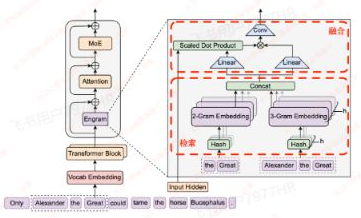
\includegraphics[width=0.98\linewidth,height=0.82\textheight,keepaspectratio]{images/DeepSeek-V4.1-Flash架构/fig-289.png}\par Engram 原文架构示意图\end{center}
\end{tcolorbox}
% source-block: 290 doxcnd0ZI3Qbc6jP86SupOr3YBf grid_column
\begin{tcolorbox}[enhanced,boxrule=0pt,colback=white,colframe=white,left=0pt,right=0pt,top=0pt,bottom=0pt]
% source-block: 291 doxcnNrOnb5Xjg0xY3ovJ6n6Lwg image
\begin{center}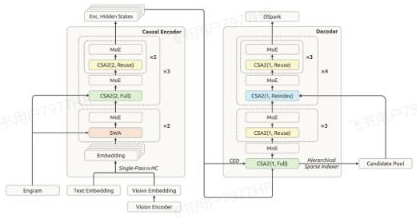
\includegraphics[width=0.98\linewidth,height=0.82\textheight,keepaspectratio]{images/DeepSeek-V4.1-Flash架构/fig-291.png}\par DeepSeek V4.1 Flash 架构\end{center}
\end{tcolorbox}
\end{tcbraster}
\end{feishuquote}

% source-block: 133 doxcnaceQppVok6TSSdWrWeKe8g callout
\begin{feishubox}{callGreen}{🧭}

% source-block: 292 doxcnyEBS0hsgqH6LU2NQ3tVeqd text
\textcolor{feishuRed}{\textbf{Engram：在标准的 Transformer 主干结构上增加 Engram 条件记忆模块，}}通过残差连接将Engram串联到 Transformer-Block主干网络：$H^{(\ell)}\leftarrow H^{(\ell)}+Y$，\textcolor{feishuRed}{注意模型结构中只有部分 Transformer-Block 增加 Engram 模块。}\par

% source-block: 293 doxcnNNSfEKPqF7TVNbmQHjqx1f text
增加 Engram 模块后，在架构上静态模式存储（Engram）与动态计算（Attention、FFN）分离。\par

% source-block: 294 doxcn8f9WpJoTxnwzxciASI0qsc text
\textcolor{feishuRed}{\textbf{新的模型结构处理每一个位置}}$t$\textcolor{feishuRed}{\textbf{的 token 方法分为两个阶段：}}给定一个输入序列 $X=(x_1,...,x_T)$ 以及第 $\ell$ 层的隐藏状态 $H^{(\ell)}\in\mathbb{R}^{T\times d}$，Engram\textcolor{feishuRed}{\textbf{ }}模块通过\textcolor{feishuRed}{检索和融合两个阶段}处理每个位置 $t$的特征：\par
\begin{itemize}
\item 
% source-block: 295 doxcnBJaHT6Kp9pvDnQqrxBiIXg bullet
\textbf{检索：}把后缀 n-gram 的 token id 压缩成规范 id，经多头哈希查嵌入表，得到记忆向量 $e_t$。\par
\item 
% source-block: 296 doxcn9pOTgj8tjU64jxlS36bPig bullet
\textbf{融合：}以隐藏状态 $h_t$ 为 query、$W_K e_t$ 为 key 算出门控 $\alpha_t$，对 value $W_V e_t$ 加权后写回。原论文在写回前还经过一层短卷积，这里 DeepSeek-V4.1-Flash 相对原始 Engram 设计去掉了短因果卷积，理由是收益不足以抵消推理栈上的复杂度。\par
\end{itemize}
\end{feishubox}

% source-block: 134 doxcn1Y63XXjA8HZWos3fZVilxf heading3
\par\Needspace{8\baselineskip}\vspace{0.8em}\noindent \begin{tcolorbox}[boxrule=0pt,arc=3pt,colback=callOrange,left=3pt,right=3pt,top=2pt,bottom=2pt,before skip=0pt,after skip=0pt]{\zihao{3}\bfseries \textcolor{feishuBlue}{3.1}\ 两个 Engram 模块的位置}\end{tcolorbox}\par\vspace{0.28em}

% source-block: 135 doxcnvQ3y6ZHL7OukVGCCMTIFXc text
Engram 以每个位置结尾的 n-gram 为 Key 查询嵌入表，取回的记忆向量经门控写回残差流，本质上是静态知识的检索，因此不再占用 Attention 与 FFN 的计算。\par

% source-block: 136 doxcnMoM1nc1ptqV6zzsw87N8ad text
V4.1-Flash 在第 1 层和第 14 层（层计数从 0 开始）各放一个 Engram 模块，合计 196B 参数（196B 的 Engram 参数均分给两个模块），不计入 552B 主干网络参数。选择这两个层插入位置的原因是让显存占用在训练流水线各段间均衡。每个模块用 $\{2,3,4\}$ 三阶 n-gram、每阶 8 个 hash head、每阶总嵌入维度 2048（ \incode{engram\_head\_dim} 乘 \incode{engram\_n\_heads} 是 256 x 8 = 2048）：\par

% source-block: 137 doxcnPvuM9jEpqQZQQQn6cQgMGh code
% Code block omitted at user request.

% source-block: 138 doxcnsWZErlXEJdz08IxSGFFWHl text
这部分参数按 n-gram 命中稀疏访问，逐 token 计算几乎不增加，代价是嵌入表放不进显存，需要依靠确定性寻址从主机内存预取。\par

% source-block: 139 doxcnG9CgmLrDfz5wdvUg9wjlnt heading3
\par\Needspace{8\baselineskip}\vspace{0.8em}\noindent \begin{tcolorbox}[boxrule=0pt,arc=3pt,colback=callOrange,left=3pt,right=3pt,top=2pt,bottom=2pt,before skip=0pt,after skip=0pt]{\zihao{3}\bfseries \textcolor{feishuBlue}{3.2}\ 检索：多头哈希查表}\end{tcolorbox}\par\vspace{0.28em}

% source-block: 140 doxcnEaxdjIjzjru6QkE4oCwWvd text
下面直接复用\href{https://scnajei2ds6y.feishu.cn/wiki/JwXTw0oUeimyoBk2QIgcSfBfn9g}{Engram：Conditional Memory via Scalable Lookup}中的符号表示：\par
\begin{itemize}
\item 
% source-block: 141 doxcnUBEBbOdVWmveI3WjK2472b bullet
$g_{t,n}$ 是以位置 $t$ 结尾、长度为 $n$ 的 n-gram，token id 已经过分词器压缩。\par
\item 
% source-block: 142 doxcnW5yfB2mBqMS3lqqk3jZy9b bullet
$\phi_{n,k}$ 是第 $n$ 阶第 $k$ 个头的哈希函数，$z_{t,n,k}$ 是哈希得到的行号。\par
\item 
% source-block: 143 doxcnI0X2KmHU19oXw8tw9RTKzd bullet
$E_{n,k}$ 是对应的嵌入表，$e_t$ 是所有头拼接后的记忆向量。\par
\end{itemize}

% source-block: 144 doxcnnPRGdA2HwbXqEZ7dN5fLLc text
\textcolor{feishuRed}{\textbf{检索阶段要解决的问题：}}n-gram 的组合数随阶数指数增长，为每个组合简历 Embedding 参数量会造成爆炸。\par

% source-block: 145 doxcn9FXAUPe73R94pYjVmXV5sb text
\textcolor{feishuRed}{\textbf{解决方法}}\textcolor{feishuRed}{：}\par
\begin{enumerate}
\item 
% source-block: 146 doxcnWrmKs5SHGR9BGC5obuhV3c ordered
\textbf{哈希降维（解决组合参数爆炸）}：$g_{t,n}$ 经 $\phi_{n,k}$ 映射到固定大小表内的行号，查表后拼接：$z_{t,n,k}\triangleq\phi_{n,k}(g_{t,n})$，$e_{t,n,k}=E_{n,k}[z_{t,n,k}]$，$e_t\triangleq\Vert_{n=2}^{N}\Vert_{k=1}^{K}e_{t,n,k}$\par
\item 
% source-block: 147 doxcnUsa3Xss3ngLt0YmbK41Mbf ordered
\textbf{多头（解决哈希冲突）}：每阶用 $K$ 个头，各自使用一张表长为不同质数的表，减少两个不同的 n-gram 在全部 K 个表上完全一致（冲突）的可能性。\par
\end{enumerate}

% source-block: 148 doxcntz3iXHEe3UxTrc47mSvpPb quote_container
\begin{feishuquote}

% source-block: 297 doxcn6LG8VUP89UaOSkBTgErZbc text
V4.1-Flash 的配置：\par
\begin{itemize}
\item 
% source-block: 298 doxcnE7bQytGIU5eM6yiAI1Fv3f bullet
$N=4$（\incode{engram\_max\_ngram\_size}），$n$ 取 2、3、4 三阶，原论文 Engram-27B 是 $N=3$。\par
\item 
% source-block: 299 doxcn96T9sFK2mnfQg1JQVqtTxc bullet
$K=8$（\incode{engram\_n\_heads}），每个模块共 $(N-1)\times K=3\times8=24$ 张表。\par
\item 
% source-block: 300 doxcnv5DseL5en0Z9WS3gLSkElf bullet
$e_{t,n,k}\in\mathbb{R}^{256}$（\incode{engram\_head\_dim}），每阶 $8\times256=2048$ 维，三阶拼接后 $e_t\in\mathbb{R}^{6144}$。\par
\item 
% source-block: 301 doxcn0NDqXfFFn9yxu73TmbRAgf bullet
分词器压缩后剩 99092 个规范 id（\incode{engram\_compressed\_vocab\_size}），规范化参考 \href{https://scnajei2ds6y.feishu.cn/wiki/JwXTw0oUeimyoBk2QIgcSfBfn9g}{Engram：Conditional Memory via Scalable Lookup}。\par
\end{itemize}
\end{feishuquote}

% source-block: 149 doxcnnNY5puGl3qtzuB7eNXUESe text
$\phi_{n,k}$ 的实现与原 Engram 相同：各阶规范 id 乘上本层的奇数乘子，逐位异或，再对第 $k$ 个头的质数表长取模。\par

% source-block: 150 doxcnmp0XoP9KVp6b8LtWJJxzVc text
V4.1 实现可以从参考\incode{NgramHashState.forward}：\par

% source-block: 151 doxcnrH2ZbIVMXYF1cWrk6Tcmsb code
% Code block omitted at user request.

% source-block: 152 doxcn7g7G2WeGPYuRiycHX0nMTf text
表长的取法：每个头的表长是互不重复的质数，从 \incode{engram\_vocab\_size} 减 1 开始用 \incode{find\_next\_prime} 逐个取下一个未用过的质数，每张约 16M 行，对应 \incode{EngramLayout.from\_args}：\par

% source-block: 153 doxcnIFTArJ9FyFJUxi3FhIm7Ee code
% Code block omitted at user request.

% source-block: 154 doxcn27P8bwgbdJ9nazNlsBaWNh text
两个模块共 48 张表，按模块求和就是 \incode{engram\_num\_embeddings} 的 384006168 与 384016682。合计 768022850 行，每行 256 维，约 196.6B 参数，即论文中的 196B。\par

% source-block: 155 doxcn8r3Io08mQ7wNHaliyMHi5b heading3
\par\Needspace{8\baselineskip}\vspace{0.8em}\noindent \begin{tcolorbox}[boxrule=0pt,arc=3pt,colback=callOrange,left=3pt,right=3pt,top=2pt,bottom=2pt,before skip=0pt,after skip=0pt]{\zihao{3}\bfseries \textcolor{feishuBlue}{3.3}\ 融合：多分支门控写回}\end{tcolorbox}\par\vspace{0.28em}

% source-block: 156 doxcn2CjZdnMUo1LQVNCPgrkhWW quote_container
\begin{feishuquote}

% source-block: 302 doxcnbU4oWnxgfDyI5Z9a6MfNwg text
单条残差流的门控可以写成 $h_t$ 与 key 的归一化内积后 sigmoid：$\alpha_t=\sigma\left(\frac{\mathrm{RMSNorm}(h_t)^\top\mathrm{RMSNorm}(k_t)}{\sqrt{d}}\right)$，最终输出为：$\tilde{v}_t=\alpha_t\cdot v_t$。\par
\end{feishuquote}

% source-block: 157 doxcn1EhfFli9uDu1P3tfKffUkg text
DeepSeek-V4.1-Flash 的残差流经 mHC 加宽成 $M=4$ 路（\incode{hc\_mult}），使用 \href{https://scnajei2ds6y.feishu.cn/wiki/JwXTw0oUeimyoBk2QIgcSfBfn9g}{Engram：Conditional Memory via Scalable Lookup}中多分支集成的版本（对照上面的单条残差流的门控理解）：\par

% source-block: 158 doxcn52hBR698WhbTjm0BWsJv2e text
\bigmath{\alpha_t^{(m)}=\sigma\left(\frac{\mathrm{RMSNorm}(\mathbf{h}_t^{(m)})^\top\mathrm{RMSNorm}(\mathbf{W}_K^{(m)}\mathbf{e}_t)}{\sqrt{d}}\right),\quad\mathbf{u}_t^{(m)}=\alpha_t^{(m)}\cdot(\mathbf{W}_V\mathbf{e}_t)}
\begin{itemize}
\item 
% source-block: 159 doxcn5tNp5rCIOCtw9cZGta6rlh bullet
$\mathbf{h}_t^{(m)}$ 是第 $m$ 条残差流在位置 $t$ 的隐藏状态，$d=5120$。\par
\item 
% source-block: 160 doxcnOCN858t8nQYCaaZME6IlCj bullet
$\mathbf{W}_K^{(m)}$ 每条流一份，每条流各自判断是否写入这条记忆。\par
\item 
% source-block: 161 doxcncZq3VSIAau2xjIprXR23nd bullet
$\mathbf{W}_V$ 四条流共用，写入的内容是同一份。\par
\end{itemize}

% source-block: 162 doxcn387FwPOMpeVJa0qsYNObwf quote_container
\begin{feishuquote}

% source-block: 303 doxcnib1a6pU5ct0Ryux59pf7e1 text
V4.1 工程上把 1 个 $\mathbf{W}_V$ 与 $M$ 个 $\mathbf{W}_K^{(m)}$ 合并成\incode{wkv} ，单次矩阵乘法获取 \incode{key} 与 \incode{value}。\par
\end{feishuquote}

% source-block: 163 doxcnNWTXcm0mss0aDTzpkRJgOb text
对应到 \incode{Engram.forward}：先查表拼接得到 $\mathbf{e}_t$，经 \incode{wkv} 切出 \incode{key} 与 \incode{value}，按流算归一化内积与 gate，最后每条流加上同一份 value 乘 gate：\par

% source-block: 164 doxcnXInLy2sSZPlK5l756rYKAb code
% Code block omitted at user request.

% source-block: 165 doxcnuaejO8TaBoV1OCoBAZZvPh text
需要注意的两个细节：\par
\begin{itemize}
\item 
% source-block: 166 doxcnD9CTFU91AoxaUw6U4mY8mf bullet
两个 RMSNorm 的缩放权重 \incode{q\_weight} 与 \incode{k\_weight} 在内积中逐元素相乘。\par
\item 
% source-block: 167 doxcnI5g0IJVbgL6ZqaBw0eMYab bullet
DeepSeek-V4.1-Flash 是多模态大模型，图像输入的 token 位置经 \incode{token\_mask} 把 gate 置零，恒等通过。\par
\end{itemize}

% source-block: 168 doxcn3daCS663UPcmw5saHy5p6r text

% source-block: 169 doxcnqAqvfPfP3feaCwZom5TnVy heading2
\par\Needspace{26\baselineskip}\vspace{0.8em}\noindent \begin{tcolorbox}[boxrule=0pt,arc=3pt,colback=callRed,left=3pt,right=3pt,top=2pt,bottom=2pt,before skip=0pt,after skip=0pt]{\zihao{-2}\bfseries \textcolor{feishuBlue}{4.}\ 其他细节改动}\end{tcolorbox}\par\vspace{0.28em}

% source-block: 170 doxcnO718QU49m6vUTpcYjUt1bb heading3
\par\Needspace{24\baselineskip}\vspace{0.8em}\noindent \begin{tcolorbox}[boxrule=0pt,arc=3pt,colback=callOrange,left=3pt,right=3pt,top=2pt,bottom=2pt,before skip=0pt,after skip=0pt]{\zihao{3}\bfseries \textcolor{feishuBlue}{4.1}\ Single-Pass mHC 与 Mega-mHC}\end{tcolorbox}\par\vspace{0.28em}

% source-block: 171 doxcnNa9BT5VfIKM1CYIr98V44c image
\begin{center}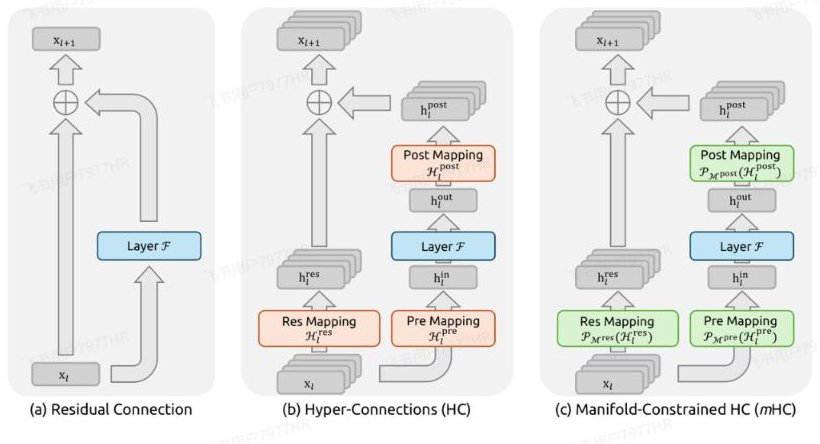
\includegraphics[width=0.98\linewidth,height=0.82\textheight,keepaspectratio]{images/DeepSeek-V4.1-Flash架构/fig-171.png}\end{center}

% source-block: 172 doxcnG6wCNfQLd13kQBWUPoQwud text
\textcolor{feishuRed}{\textbf{动机：}} mHC 把残差流拆成 $n$ 份并行副本，块间更新式是 $\mathbf{x}_{l+1}=\mathcal{H}_{l}^{res}\mathbf{x}_l+\mathcal{H}_{l}^{post\top}\mathcal{F}(\mathcal{H}_{l}^{pre}\mathbf{x}_l,\mathcal{W}_l)$，$(\mathcal{H}_l^{pre},\mathcal{H}_l^{res},\mathcal{H}_l^{post})=\mathcal{H}(X_l)$。理想情况下中间激活访存下界为 $(2n+2)d$，而 DeepSeek V4 的实现是三个串行 kernel，因为 $\hat{\mathbf{x}}_l=\mathcal{H}_l^{pre}\mathbf{x}_l$ 要等 $\mathcal{H}(X_l)$ 在隐藏维上求和完成，合计 $(4n+4)d$，开销是下界的两倍。\par

% source-block: 173 doxcnnBchjdN052tCjIj2aWpUje callout
\begin{feishubox}{callGreen}{📌}

% source-block: 304 doxcnnu9H1Bb9LhUgYTfrJN0mAe text
对应到 \href{https://my.feishu.cn/wiki/WsaawrdO3ifrmTk3ab4cSgjBnRb}{mHC：Manifold-Constrained Hyper-Connections}的符号系统，每个子层的更新式为 $\mathbf{x}_{l+1}=\mathcal{H}_{l}^{res}\mathbf{x}_l+\mathcal{H}_{l}^{post\top}\mathcal{F}(\mathcal{H}_{l}^{pre}\mathbf{x}_l,\mathcal{W}_l)$。\par

% source-block: 305 doxcnBpi3P8zwVNJ65PsIQV5Ffd text
理想情况下，相邻两个子层之间的残差变换是一个映射。\par

% source-block: 306 doxcntpTJvHZPzFB3ve0MvKISxf text
这个映射的输入是上一子层的残差流 $\mathbf{x}_{l-1}$ 与子层输出 $\mathbf{y}_{l-1}=\mathcal{F}(\hat{\mathbf{x}}_{l-1},\mathcal{W}_{l-1})$，输出是本层残差流 $\mathbf{x}_l$ 与本层子层输入 $\hat{\mathbf{x}}_l=\mathcal{H}_l^{pre}\mathbf{x}_l$。\par

% source-block: 307 doxcnoxQZTcxn9dhFpo0TJ4DBWd text
用激活访存量（activation memory traffic）衡量这次变换的开销，即每个 token 读、写的激活元素数。理想映射读入前两者、写出后两者，读 / 写各 $(n+1)d$，下界是 $(2n+2)d$。\par

% source-block: 308 doxcnXajbcfO7gdcuprR82jXmqh text
DeepSeek V4 受数据依赖限制，把这个映射拆成三个串行 kernel：\par

% source-block: 309 doxcn7bxSaN4yYEmMkWYZ38ZLRe text
\bigmath{\mathbf{x}_l=\mathcal{H}_{l-1}^{res}\mathbf{x}_{l-1}+\mathcal{H}_{l-1}^{post\top}\mathbf{y}_{l-1},\quad(\mathcal{H}_l^{pre},\mathcal{H}_l^{post},\mathcal{H}_l^{res})=\mathcal{H}(\mathbf{x}_l),\quad\hat{\mathbf{x}}_l=\mathcal{H}_l^{pre}\mathbf{x}_l}
\begin{itemize}
\item 
% source-block: 310 doxcn9O0KRgcDWkEP7FQ4XIjmMg bullet
第一个 kernel 是残差更新，即 $\mathcal{F}_{\mathrm{post},\mathrm{res}}$，读 $(n+1)d$、写 $nd$。\par
\item 
% source-block: 311 doxcnOOwGF3NPi2xnluxEGNpUpf bullet
第二个 kernel 是系数预测，要在全部 $nd$ 个元素上归约，读 $nd$。\par
\item 
% source-block: 312 doxcnh5TDHr2uCBY9jfzc91tTnc bullet
第三个 kernel 是输入混合，即 $\mathcal{F}_{\mathrm{pre}}$，在各条流上归约，读 $nd$、写 $d$。\par
\end{itemize}

% source-block: 313 doxcnvrqhGJC3YU9sv3lBF21GFc text
再算上子层 pre-norm 读写各 $d$，合计 $(4n+4)d$，为下界 $(2n+2)d$ 的两倍。\par
\end{feishubox}

% source-block: 174 doxcnXQWk9zXA2AQdoAdV6k6d8d text
\textcolor{feishuRed}{\textbf{实现：}} 把读所用的系数错开（位移）一个子层，每个子层使用上一子层预测的 $\mathcal{H}^{pre}$：\par

% source-block: 175 doxcn4lxooBdqMtd47pSFXq2qYu text
\bigmath{\mathbf{x}_{l+1}=\mathcal{H}_l^{res}\mathbf{x}_l+\mathcal{H}_l^{post\top}\mathcal{F}(\mathcal{H}_{l-1}^{pre}\mathbf{x}_l,\mathcal{W}_l),\quad(\mathcal{H}_l^{pre},\mathcal{H}_l^{post},\mathcal{H}_l^{res})=\mathcal{H}(\mathbf{x}_l)}

% source-block: 176 doxcnmAfAYmWib7IxTPnQqOIglC text
其中 $\mathcal{H}_{l-1}^{pre}$ 由上一子层的残差流预测，本子层开始计算之前已就绪，本子层预测出的 $\mathcal{H}_{l}^{pre}$ 留给下一子层，并且 V4.1 认为这一位移的性能退化可忽略。\par

% source-block: 177 doxcnDxBoQH6IFFzq4cLGPWqqjb text
预训练仍用多 kernel 实现，推理部署侧把残差更新、输入混合、系数预测融进单个 Mega-mHC kernel，达到 $(n+1)d$ 读 / $(n+1)d$ 写的理论值。位移在 \incode{Block.forward} 的实现：\par

% source-block: 178 doxcnxENNrrN0odrC64XV7ZY9kh code
% Code block omitted at user request.

% source-block: 179 doxcnCcFyHt3pjLy7cAkyAQVtXb text

% source-block: 180 doxcnOaAxyaOoulVMwnrSjuw3Gb heading3
\par\Needspace{8\baselineskip}\vspace{0.8em}\noindent \begin{tcolorbox}[boxrule=0pt,arc=3pt,colback=callOrange,left=3pt,right=3pt,top=2pt,bottom=2pt,before skip=0pt,after skip=0pt]{\zihao{3}\bfseries \textcolor{feishuBlue}{4.2}\ FP4 Main KV Cache}\end{tcolorbox}\par\vspace{0.28em}

% source-block: 181 doxcnR0bEfWFghwSfxlBUSHI5Qd text
\textcolor{feishuRed}{\textbf{动机：}} DeepSeek V4 已经对 indexer 的 Q 与 K 做 FP4 QAT，但是 main KV 还是 FP8，而长程 agent 负载下 per-request 的 KV 体积直接决定并发。\par

% source-block: 182 doxcnI8fV1kcH9WT2TBJPD5BVlb text
\textcolor{feishuRed}{\textbf{实现：}} 采用 OCP 标准的 MXFP4（E2M1 + 每 16 通道一个 E4M3 scale），去掉 NVFP4 的二级全局 scale。\par

% source-block: 183 doxcn151a1gJbKVz3nGJ0KeC2yd code
% Code block omitted at user request.

% source-block: 184 doxcn5r3IQlgnbUWN27eNYcdrLx text

% source-block: 185 doxcnqC2JCe1pVbcmXcvJv3sGqg heading3
\par\Needspace{8\baselineskip}\vspace{0.8em}\noindent \begin{tcolorbox}[boxrule=0pt,arc=3pt,colback=callOrange,left=3pt,right=3pt,top=2pt,bottom=2pt,before skip=0pt,after skip=0pt]{\zihao{3}\bfseries \textcolor{feishuBlue}{4.3}\ DSpark}\end{tcolorbox}\par\vspace{0.28em}

% source-block: 186 doxcnkzO2pUL5KooEiKEdQgqZ2K text
V4.1-Flash 使用的 Speculative Decoding 模块是 DSpark。DSpark 具体技术参考 \href{https://my.feishu.cn/wiki/J3Diws4MwiYVT9ksYhLcU6jtnLe}{从 Speculative 到 DSpark：拆解 DeepSeek 推测解码}、\href{https://my.feishu.cn/wiki/KwlAwvEHKilNdXkbaz5cTMagnHe}{推测解码对比解析：DeepSeek-DSpark / 阶跃-JetSpec}。\par

% source-block: 187 doxcn26Ly7dXcORqU8FxjMggnIb callout
\begin{feishubox}{callOrange}{🌟}

% source-block: 314 doxcnXylJrDvAZaBdiR7X3Qt8gh text
DSpark 同时改进了推测解码（Speculative Decoding）的 \textbf{Drafting} 和 \textbf{Verification} 两侧的效率：\par

% source-block: 315 doxcnttJxtLwVtHcSrtrqiZPmOf text
\textbf{Drafting：}用\textcolor{feishuRed}{\textbf{\incode{半自回归生成}}}平衡了并行 drafter（DFlash）的低延迟 \& 自回归 drafter 的高接受率。\par

% source-block: 316 doxcnH03Riz3qGKlmisdp0YMRib text
\textbf{Verification：}训练\textcolor{feishuRed}{\textbf{\incode{置信 head}}}预测每一个位置的接受率、结合\textcolor{feishuRed}{\textbf{\incode{硬件感知的调度算法}}}截断验证长度。\par

% source-block: 317 doxcnswaAalB0TzABDSBar7FXQ8 text
两者共同改进了推测解码的效率，即有效 token 的输出延迟。\par
\end{feishubox}

% source-block: 188 doxcnIyIJl6lxEOGMUB1r2WascK text
训练设置与 DeepSeek V3 的 MTP 相反：MTP 在预训练全程与主干联合训练，DSpark 则在预训练之后单独阶段训练、主干冻结。后训练阶段两者同时训练但不向主干回传梯度，既能加速在线服务也能加速 RL 与 OPD 的 rollout 生成，相关配置对应到 \incode{config.json}：\par

% source-block: 189 doxcn2Y54vxMNZdbFWLPOW4z4i1 code
% Code block omitted at user request.

% source-block: 190 doxcngdtvtOJaeUqPkgbnav4E6U text

% source-block: 191 doxcn6zoH4AAIozX25Wcff7mCwb heading3
\par\Needspace{43\baselineskip}\vspace{0.8em}\noindent \begin{tcolorbox}[boxrule=0pt,arc=3pt,colback=callOrange,left=3pt,right=3pt,top=2pt,bottom=2pt,before skip=0pt,after skip=0pt]{\zihao{3}\bfseries \textcolor{feishuBlue}{4.4}\ DeepSeek-ViT / 多模态负载均衡}\end{tcolorbox}\par\vspace{0.28em}

% source-block: 192 doxcnLfF2UP7ds5Ztr0ci0sPOHf grid
\begin{tcbraster}[raster columns=2,raster equal height=rows,raster column skip=8pt,raster row skip=8pt,raster left skip=0pt,raster right skip=0pt]

% source-block: 318 doxcnkELl3uhccc79P35GlaC8Vc grid_column
\begin{tcolorbox}[enhanced,boxrule=0pt,colback=white,colframe=white,left=0pt,right=0pt,top=0pt,bottom=0pt]
% source-block: 319 doxcnnZiDaudyXCs7bOfNJle5ah text
Vision Encoder 是从头训练的 DeepSeek-ViT：32 层、隐藏维度 1024、16 head、patch 14。相对标准 \href{https://scnajei2ds6y.feishu.cn/wiki/QEJ8wXq9GiTBrxkMqbScnd8nnod}{ViT(2020, Google Research)} 的三处改动：\par
\begin{itemize}
\item 
% source-block: 320 doxcnckWbiD25k0P8TgAckcW3vh bullet
绝对位置编码换成 2D-RoPE 以支持任意分辨率。\par
\item 
% source-block: 321 doxcnzl9K0ifv9KDXmhfxksERXb bullet
Patch Embedding 的卷积换成线性投影以兼容 Muon。\par
\item 
% source-block: 322 doxcnxZ1kqEkUgNpLEo7nyniLDc bullet
归一化与激活改用 RMSNorm 与 SwiGLU。\par
\end{itemize}
% source-block: 323 doxcnmtjCWbJh2IkSMJdqGuIdCh text
比较值得注意的是 Projection 使用 $3\times3$ 的 pixel-unshuffle，相比现在常用的 $2\times2$ 有更高的压缩比：\par
\end{tcolorbox}
% source-block: 324 doxcniiBfJw6X37ogz1yf4LB2Le grid_column
\begin{tcolorbox}[enhanced,boxrule=0pt,colback=white,colframe=white,left=0pt,right=0pt,top=0pt,bottom=0pt]
% source-block: 325 doxcnTqYR2ymI2RtrWkbghQJrCe image
\begin{center}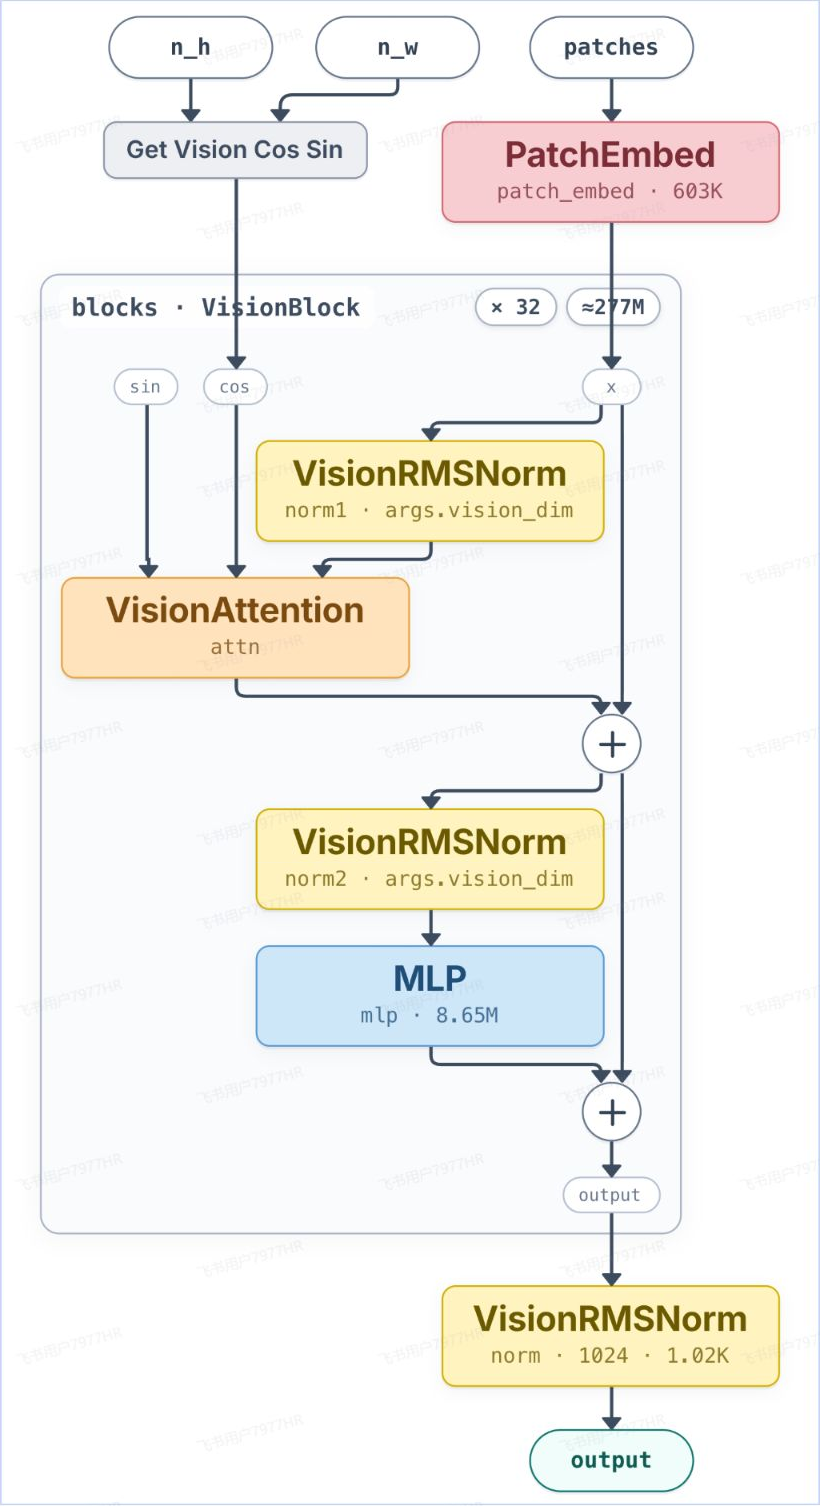
\includegraphics[width=0.98\linewidth,height=0.82\textheight,keepaspectratio]{images/DeepSeek-V4.1-Flash架构/fig-325.png}\end{center}
\end{tcolorbox}
\end{tcbraster}

% source-block: 193 doxcndTwxEZ6xDnUTGa9tteUIbc grid
\begin{tcbraster}[raster columns=2,raster equal height=rows,raster column skip=8pt,raster row skip=8pt,raster left skip=0pt,raster right skip=0pt]

% source-block: 326 doxcnSRBami1GPa3XKsVx4gsJgc grid_column
\begin{tcolorbox}[enhanced,boxrule=0pt,colback=white,colframe=white,left=0pt,right=0pt,top=0pt,bottom=0pt]
% source-block: 327 doxcnpdrlpUuSoapBiZVYNM9arb code
% Code block omitted at user request.
\end{tcolorbox}
% source-block: 328 doxcnI5bEDIQGQCw5rik1HGg0og grid_column
\begin{tcolorbox}[enhanced,boxrule=0pt,colback=white,colframe=white,left=0pt,right=0pt,top=0pt,bottom=0pt]
% source-block: 329 doxcnMwv3MUdgzV9n5cP7hyYqqu image
\begin{center}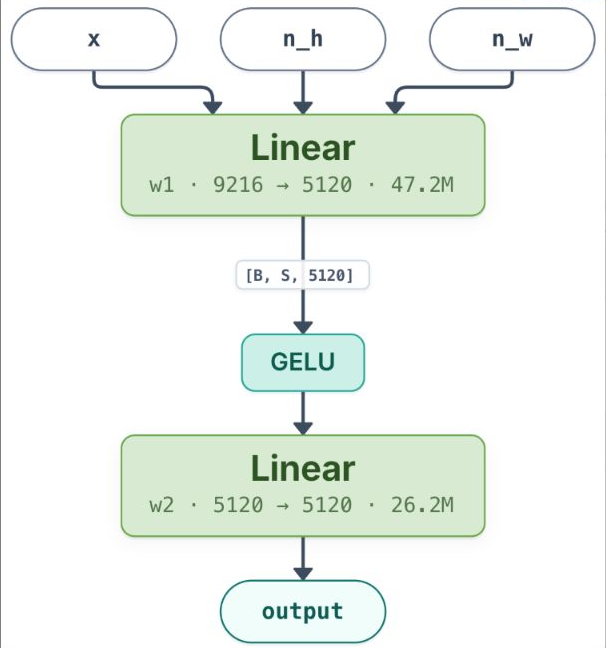
\includegraphics[width=0.98\linewidth,height=0.82\textheight,keepaspectratio]{images/DeepSeek-V4.1-Flash架构/fig-329.png}\par Aligner 架构\end{center}
\end{tcolorbox}
\end{tcbraster}

% source-block: 194 doxcnq4ZOGLXf0hA5CvQoLQi2Ph quote_container
\begin{feishuquote}
\begin{itemize}
\item 
% source-block: 330 doxcnr1mFpcPSVVwSkdYB91qX1b bullet
\incode{downsample\_ratio} 取 3，\incode{F.unfold} 把 $3\times3$ 邻域展开到通道维度。\par
\item 
% source-block: 331 doxcnJjQgLsT3hGWJMqmdcUwrvc bullet
投影器是两层 MLP，本质上就是 \href{https://scnajei2ds6y.feishu.cn/docx/H7v3dR83UobvcoxbI4UcrzvLngh}{面试官：MLLM有哪些图像token压缩方法} 里 pixel-shuffle 类操作。\par
\item 
% source-block: 332 doxcnVgMZdVhr01uHh0fkcFOD7d bullet
ViT 内 2D-RoPE 的实现参考 \href{https://scnajei2ds6y.feishu.cn/docx/PiAPdtlhxoxawvxtR5lcZGrNnT5}{2D-RoPE}。\par
\end{itemize}
\end{feishuquote}

% source-block: 195 doxcnFISI3HRTB1OcpKeeQYvQwf text
语言主干模型 MoE 侧为多模态单独做了改动：\par

% source-block: 196 doxcnwTKIGYbWzGkDGic88m9F9d text
\textcolor{feishuRed}{\textbf{动机：}}图像与文本 token 的表示分布与路由偏好都不同，把两者的负载合起来均衡会掩盖模态内部的不均衡。\par

% source-block: 197 doxcnIRnHWPdwthkz746at9TALg text
\textcolor{feishuRed}{\textbf{实现：}}把 auxiliary-loss-free 的 correction bias 拆成两套，文本与图像单独做专家选择，路由权重仍取自未加 bias 的原始分数，两套按各自负载独立更新。\par

% source-block: 198 doxcn5J7BQswe9PT5tA9fgjGCEh text

% source-block: 199 doxcnFyOhksINMshtB62iNKWppg heading3
\par\Needspace{8\baselineskip}\vspace{0.8em}\noindent \begin{tcolorbox}[boxrule=0pt,arc=3pt,colback=callOrange,left=3pt,right=3pt,top=2pt,bottom=2pt,before skip=0pt,after skip=0pt]{\zihao{3}\bfseries \textcolor{feishuBlue}{4.5}\ Optimizer}\end{tcolorbox}\par\vspace{0.28em}
\begin{itemize}
\item 
% source-block: 200 doxcntbYzCiX5us5I8wezgyNzzb bullet
Head-wise Muon：权重按 head 切开再各自更新，以处理 head 之间的异质性，细节参考 \href{https://scnajei2ds6y.feishu.cn/wiki/Hcj2wGTJEiohTikkdEKc7H4Nnlb}{Muon 优化器}。\par
\item 
% source-block: 201 doxcnFnqg3xqWUMWJl2DPIWopih bullet
Engram 改成动量更新 + Sinkhorn balancing：把 Muon 里的 Newton-Schulz 正交化换成对更新矩阵做行列交替 RMSNorm（迭代次数$K=11$ 步）。\par
\end{itemize}

% source-block: 202 doxcnFANeoXxPakZdhti4geWcPc text

% source-block: 203 doxcnf2Hmv4sOAsyRaq7C2EddId text

\end{document}
